\documentclass[10pt,a4paper,onecolumn]{article}
% \usepackage[utf8]{inputenc}
\usepackage{marginnote}
\usepackage{graphicx}
\usepackage{xcolor}
\usepackage{authblk,etoolbox}
\usepackage{titlesec}
\usepackage{calc}
\usepackage{hyperref}
\hypersetup{breaklinks=true,
            bookmarks=true,
            pdfauthor=
{
      Simen Tennøe,
      Kjetil Hodne,
      Trude M. Haug,
      Finn-Arne Weltzien,
      Gaute T. Einevoll,
      Geir Halnes,
  },
            pdftitle=
{
[Re] Fast-Activating Voltage- and Calcium-Dependent Potassium (BK)
Conductance Promotes Bursting in Pituitary Cells: A Dynamic Clamp Study
},
            colorlinks=true,
            citecolor=blue,
            urlcolor=blue,
            linkcolor=blue,
            pdfborder={0 0 0}}
\urlstyle{same}
\usepackage{tcolorbox}
\usepackage{ragged2e}
\usepackage{fontspec}
\usepackage{fontawesome}
\usepackage{caption}
\usepackage{listings}
\lstnewenvironment{code}{\lstset{language=Haskell,basicstyle=\small\ttfamily}}{}



%\usepackage{fancyvrb}
%\VerbatimFootnotes
%\usepackage{graphicx}
%\usepackage{mdframed}
%\newmdenv[backgroundcolor=lightgray]{Shaded}


\usepackage{longtable,booktabs}

\usepackage[
  backend=biber,
%  style=alphabetic,
%  citestyle=numeric
]{biblatex}
\bibliography{bibliography.bib}



% --- Macros ------------------------------------------------------------------
\renewcommand*{\bibfont}{\small \sffamily}

\definecolor{red}{HTML}{CF232B}
\newcommand{\ReScience}{Re{\bfseries \textcolor{red}{Science}}}

\newtcolorbox{rebox}
   {colback=blue!5!white, colframe=blue!40!white,
     boxrule=0.5pt, arc=2pt, fonttitle=\sffamily\scshape\bfseries,
     left=6pt, right=20pt, top=6pt, bottom=6pt}

\newtcolorbox{repobox}
   {colback=red, colframe=red!75!black,
     boxrule=0.5pt, arc=2pt, left=6pt, right=6pt, top=3pt, bottom=3pt}

% fix for pandoc 1.14     
\newcommand{\tightlist}{%
  \setlength{\itemsep}{1pt}\setlength{\parskip}{0pt}\setlength{\parsep}{0pt}}

% --- Style -------------------------------------------------------------------
\renewcommand*{\bibfont}{\small \sffamily}
\renewcommand{\captionfont}{\small\sffamily}
\renewcommand{\captionlabelfont}{\bfseries}

\makeatletter
\renewcommand\@biblabel[1]{{\bf #1.}}
\makeatother

% --- Page layout -------------------------------------------------------------
\usepackage[top=3.5cm, bottom=3cm, right=1.5cm, left=1.5cm,
            headheight=2.2cm, reversemp, includemp, marginparwidth=4.5cm]{geometry}

% --- Section/SubSection/SubSubSection ----------------------------------------
\titleformat{\section}
  {\normalfont\sffamily\Large\bfseries}
  {}{0pt}{}
\titleformat{\subsection}
  {\normalfont\sffamily\large\bfseries}
  {}{0pt}{}
\titleformat{\subsubsection}
  {\normalfont\sffamily\bfseries}
  {}{0pt}{}
\titleformat*{\paragraph}
  {\sffamily\normalsize}


% --- Header / Footer ---------------------------------------------------------
\usepackage{fancyhdr}
\pagestyle{fancy}
%\renewcommand{\headrulewidth}{0.50pt}
\renewcommand{\headrulewidth}{0pt}
\fancyhead[L]{\hspace{-1cm}\includegraphics[width=4.0cm]{rescience-logo.pdf}}
\fancyhead[C]{}
\fancyhead[R]{} 
\renewcommand{\footrulewidth}{0.25pt}

\fancyfoot[L]{\hypersetup{urlcolor=red}
              \sffamily \ReScience~$\vert$
              \href{http://rescience.github.io}{rescience.github.io}
              \hypersetup{urlcolor=blue}}
\fancyfoot[C]{\sffamily 2 - \thepage}
\fancyfoot[R]{\sffamily Mar 2019 $\vert$
                        Volume \textbf{5} $\vert$
                        Issue \textbf{1}}
\pagestyle{fancy}
\makeatletter
\let\ps@plain\ps@fancy
\fancyheadoffset[L]{4.5cm}
\fancyfootoffset[L]{4.5cm}

% --- Title / Authors ---------------------------------------------------------
% patch \maketitle so that it doesn't center
\patchcmd{\@maketitle}{center}{flushleft}{}{}
\patchcmd{\@maketitle}{center}{flushleft}{}{}
% patch \maketitle so that the font size for the title is normal
\patchcmd{\@maketitle}{\LARGE}{\LARGE\sffamily}{}{}
% patch the patch by authblk so that the author block is flush left
\def\maketitle{{%
  \renewenvironment{tabular}[2][]
    {\begin{flushleft}}
    {\end{flushleft}}
  \AB@maketitle}}
\makeatletter
\renewcommand\AB@affilsepx{ \protect\Affilfont}
%\renewcommand\AB@affilnote[1]{{\bfseries #1}\hspace{2pt}}
\renewcommand\AB@affilnote[1]{{\bfseries #1}\hspace{3pt}}
\makeatother
\renewcommand\Authfont{\sffamily\bfseries}
\renewcommand\Affilfont{\sffamily\small\mdseries}
\setlength{\affilsep}{1em}

\LetLtxMacro{\OldIncludegraphics}{\includegraphics}
\renewcommand{\includegraphics}[2][]{\OldIncludegraphics[width=12cm, #1]{#2}}


% --- Document ----------------------------------------------------------------
\title{[Re] Fast-Activating Voltage- and Calcium-Dependent Potassium (BK)
Conductance Promotes Bursting in Pituitary Cells: A Dynamic Clamp Study}

    \usepackage{authblk}
                        \author[1, 2]{Simen Tennøe}
                    \author[3]{Kjetil Hodne}
                    \author[4]{Trude M. Haug}
                    \author[3]{Finn-Arne Weltzien}
                    \author[1, 5, 6]{Gaute T. Einevoll}
                    \author[1, 5]{Geir Halnes}
                            \affil[1]{Centre for Integrative Neuroplasticity, University of Oslo, Oslo, Norway}
                    \affil[2]{Department of Informatics, University of Oslo, Oslo, Norway}
                    \affil[3]{Department of Basic Sciences and Aquatic Medicine, Norwegian University
of Life Sciences, Campus Adamstuen, Norway}
                    \affil[4]{Institute of Oral Biology, University of Oslo, Oslo, Norway}
                    \affil[5]{Faculty of Science and Technology, Norwegian University of Life
Sciences, Ås, Norway}
                    \affil[6]{Department of Physics, University of Oslo, Oslo, Norway}
            
\date{\vspace{-5mm}
      \sffamily \small \href{mailto:simenten@student.matnat.uio.no}{simenten@student.matnat.uio.no}}


\setlength\LTleft{0pt}
\setlength\LTright{0pt}


\begin{document}
\maketitle

\marginpar{
  %\hrule
  \sffamily\small
  %\vspace{2mm}
  {\bfseries Editor}\\
  Benoît Girard\\

  {\bfseries Reviewers}\\
        Georgios Detorakis\\
        Andrew P. Davison\\
  
  {\bfseries Received}  Nov, 9, 2018\\
  {\bfseries Accepted}  Mar, 11, 2019\\
  {\bfseries Published} Mar, 21, 2019\\

  {\bfseries Licence}   \href{http://creativecommons.org/licenses/by/4.0/}{CC-BY}

  \begin{flushleft}
  {\bfseries Competing Interests:}\\
  The authors have declared that no competing interests exist.
  \end{flushleft}

  \hrule
  \vspace{3mm}

  \hypersetup{urlcolor=white}
  
    \vspace{-1mm}
  \begin{repobox}
    \bfseries\normalsize
      \href{https://github.com/ReScience-Archives/Tenn-e-Hodne-Haug-Weltzien-Einevoll-Halnes-2019/tree/tenn\%C3\%B8e-hodne-haug-weltzien-einevoll-halnes/article}{\faGithubAlt~Article repository}
  \end{repobox}
      \vspace{-1mm}
  \begin{repobox}
    \bfseries\normalsize
      \href{https://github.com/ReScience-Archives/Tenn-e-Hodne-Haug-Weltzien-Einevoll-Halnes-2019/tree/tenn\%C3\%B8e-hodne-haug-weltzien-einevoll-halnes/code}{\faGithubAlt~Code repository}
  \end{repobox}
        \hypersetup{urlcolor=blue}
}

\begin{rebox}
\sffamily {\bfseries A reference implementation of}
\small
\begin{flushleft}
\begin{itemize}
    \item[→] \emph{Fast-Activating Voltage- and Calcium-Dependent Potassium (BK)
Conductance Promotes Bursting in Pituitary Cells: A Dynamic Clamp
Study}, J. Tabak, M. Tomaiuolo, A. Gonzalez-Iglesias, L. Milescu and R.
Bertram, Journal of Neuroscience 31.46 (2011),
10.1523/JNEUROSCI.3235-11.2011
  \end{itemize}\par
\end{flushleft}
\end{rebox}


\section{Introduction}\label{introduction}

As part of the dynamic clamp study by Tabak et al. 2011
\autocite{tabak2011}, a computational model was developed for the
voltage dynamics of endocrine pituitary cells in rats. The model
captured the spontaneous activity of these cells, including the
generation of Ca\textsuperscript{2+}-channel mediated spikes and
pseudo-plateau bursts. As an important achievement, the model explained
the paradoxical role that big conductance K\textsuperscript{+} (BK)
channels had in prolonging spike duration and sometimes promoting burst
firing in these cells \autocite{vangoor2001}, contrary to what one would
expect from a hyperpolarizing current. The original model was
implemented in XPP \autocite{ermentrout2002}. The code for the model was
made available online at
\url{https://www.math.fsu.edu/~bertram/software/pituitary/JNS_11b.ode},
while the code used in the analysis of the model outcome was not made
available.

In the current paper, we have reimplemented the computational model by
Tabak et al. \autocite{tabak2011} using the Python interface for the
NEURON simulator \autocite{hines1997}, a widely used simulator for
multicompartmental neurons. In addition, we have performed an
uncertainty quantification and sensitivity analysis of the model using
the Uncertainpy Python package \autocite{uncertainpy}, version 1.1.4
(Zenodo:
\href{http://doi.org/10.5281/zenodo.1473453}{10.5281/zenodo.1473453}).
The model implementation works with Python 2 and 3. The results in this
paper were created using Python 3.7.0 within a Docker
(\url{https://www.docker.com/}) environment.

The reimplemented model reproduced the characteristic firing patterns
seen in the original publication, and we thus confirmed the original
study. The sensitivity analysis further presented a systematic overview
of the model in terms of how its characteristic response features
depended on the various model parameters. Supporting the main conclusion
from the original work, the sensitivity analysis showed that the
bursting propensity of the model was highly sensitive to the BK
conductance. However, the analysis also revealed that the bursting
propensity was sensitive to additional parameters (conductances), and
thus that BK is not the sole determinant for whether the cell is bursty.

\section{Methods}\label{methods}

When reimplementing the model by Tabak et al. \autocite{tabak2011} we
followed the descriptions in the original publication, using the
original implementation for verification purposes. We also had a brief
communication with the original authors to obtain details on the
analysis part of the model.

\subsection{Model}\label{model}

The model by Tabak et al. \autocite{tabak2011} was defined by the
equation:

\begin{equation}C \frac{dV}{dt} = - (I_{\mathrm{Ca}} + I_{\mathrm{K}} + I_{\mathrm{BK}} + I_{\mathrm{SK}} + I_{\mathrm{leak}} + I_{\mathrm{noise}} ),\label{eq:V}\end{equation}

\noindent
where \(C\) is the membrane capacitance, \(V\) is the membrane
potential, and \(I_X\) the current through a specific ion channel \(X\).
The model included six different currents:

\begin{itemize}
\tightlist
\item
  \(I_{\mathrm{Ca}}\) -- Voltage gated Ca\textsuperscript{2+} current.
\item
  \(I_{\mathrm{K}}\) -- Voltage gated K\textsuperscript{+} current.
\item
  \(I_{\mathrm{BK}}\) -- Big conductance K\textsuperscript{+} current.
\item
  \(I_{\mathrm{SK}}\) -- Small conductance K\textsuperscript{+} current.
\item
  \(I_{\mathrm{leak}}\) -- Leak current.
\item
  \(I_{\mathrm{noise}}\) -- Stochastic current representing channel
  noise.
\end{itemize}

\noindent
A current through an ion channel \(X\) was given by the simplified
relation:

\begin{equation}I_{X} = G_{X}Y_X(V - E_{X}),\label{eq:I}\end{equation}

\noindent
where \(G_{X}\) denotes the maximum ion channel conductance, and
\(E_{X}\) denotes the reversal potential of the ion species conducted by
channel \(X\). \(Y_X\) denotes an ion channel specific gating function,
which was unity for \(I_{\mathrm{leak}}\), an instantaneous function of
\(V\) for \(I_{\mathrm{Ca}}\), an instantaneous function of the
cytosolic Ca\textsuperscript{2+} concentration for \(I_{\mathrm{SK}}\),
and a dynamic function of \(V\) and \(t\) for the remaining ion channels
\(I_{\mathrm{K}}\), \(I_{\mathrm{BK}}\), and \(I_{\mathrm{K}}\).

The original implementation used the total membrane capacitance (units
pF) and total membrane conductances (units nS), while the NEURON
simulator requires these entities to be specified per membrane area with
units \(\mu \mathrm{F/cm}^2\) and S/cm\textsuperscript{2}, respectively.
NEURON also requires that the membrane area is defined. To get the
parameters on the form required by NEURON we defined an arbitrary
membrane area (\(A\)), and divided the capacitance \(C\) and ion channel
conductances \(G_X\) by \(A\):

\begin{equation}g_{X,\,\mathrm{NEURON}} = \frac{G_X}{A}, \qquad c_{\mathrm{NEURON}} = \frac{C}{A}.\label{eq:c_g}\end{equation}

\noindent
Combining Equation ~\ref{eq:V}, ~\ref{eq:I} and ~\ref{eq:c_g} shows that
the model is independent of the choice of \(A\):

\begin{equation}\frac{C}{A} \frac{dV}{dt} =  -\left(\frac{G_{X}}{A}Y_X(V - E_{X}) + \ldots \right).\label{eq:V_A}\end{equation}

The original model further included an equation for handling the
intracellular Ca\textsuperscript{2+} concentration, which is relevant
for the gating of SK channels:

\begin{equation}\frac{d[Ca]}{dt} = - f_c (\alpha I_{\mathrm{Ca}} + k_c[Ca]), \label{eq:Ca}\end{equation}

\noindent
where \(f_c\) denotes the fraction of free Ca\textsuperscript{2+} in the
cytoplasm, \(k_c\) denotes the extrusion rate, and the constant
\(\alpha\) converts an incoming current to a molar concentration.
\(\alpha\) was converted to NEURON units by taking:

\begin{equation}\alpha_{\mathrm{NEURON}} = A\alpha.\label{eq:alpha}\end{equation}

\noindent
Combining Equation ~\ref{eq:c_g}, ~\ref{eq:Ca} and ~\ref{eq:alpha} shows
that this choice keeps the model independent of the choice of \(A\):

\begin{equation}\frac{d[Ca]}{dt} = - f_c (A\alpha \frac{G_{\mathrm{Ca}}}{A}(V - E_{\mathrm{Ca}}) + k_c[Ca]).\label{eq:Ca_A}\end{equation}

We arbitrarily chose a cell body with a membrane area of
\(\pi \cdot 10^{-6}\) cm\textsuperscript{2}, i.e.~with a diameter of 10
\(\mu\)m. We used all equations from the original publication,
substituting \(G_X\) with \(g_{X,\,\mathrm{NEURON}}\), \(C\) with
\(c_{\mathrm{NEURON}}\), and \(\alpha\) with
\(\alpha_{\mathrm{NEURON}}\). The parameter values from the original
publication and the converted parameter values are summarized in Table
~\ref{tbl:parameters}. Parameters not listed in this table were kept
unchanged from the original publication. To make the discussion and
results easier to compare to the original publication, we will refer to
the original conductance values through the rest of this paper.

The noise was added by using a current clamp that injected a random
current at each time step in the simulation, as described by the
original publication. Simulations with noise were run with a fixed time
step of \texttt{dt\ =\ 0.01} ms, which is the same time step used in the
original publication. When performing the sensitivity analysis, the
noise amplitude was set to zero (\(A_{\mathrm{noise}} = 0\)), and the
simulations were run using adaptive time steps.

We found one discrepancy between the parameters listed in the original
publication and the values found in the original source code. The
maximum conductance of K\textsuperscript{+} channels
(\(G_{\mathrm{K}}\)) was listed as 3.2 nS in the original publication,
while the value used in the original source code was 3 nS. Both values
were tested and \(G_{\mathrm{K}} = 3\) nS gave results most similar to
the results in the original publication. We therefore decided to use
\(G_{\mathrm{K}} = 3\) nS instead of the value listed in the original
publication.

\hypertarget{tbl:parameters}{}
\begin{longtable}[]{@{}llllll@{}}
\caption{\label{tbl:parameters}The parameter values in Tabak et al.
\autocite{tabak2011} that were converted from currents and capacitance
to currents and capacitance per membrane area due to requirements by the
NEURON simulator. The original model parameter values are denoted Tabak
while the parameter values in the reimplemented model are denoted
NEURON, with names as used in the model implementation. }\tabularnewline
\toprule
Tabak & Value & Unit & NEURON & Value & Unit\tabularnewline
\midrule
\endfirsthead
\toprule
Tabak & Value & Unit & NEURON & Value & Unit\tabularnewline
\midrule
\endhead
& & & \texttt{A} & \(3.14 \cdot 10^{-6}\) &
cm\textsuperscript{2}\tabularnewline
C & 10 & pF & \texttt{c} & 3.18 & \(\mu \mathrm{F/cm}^2\)\tabularnewline
\(G_{\mathrm{Ca}}\) & 2 & nS & \texttt{g\_Ca} & \(6.37 \cdot 10^{-4}\) &
S/cm\textsuperscript{2}\tabularnewline
\(G_{\mathrm{K}}\) & 3 & nS & \texttt{g\_K} & \(9.55 \cdot 10^{-4}\) &
S/cm\textsuperscript{2}\tabularnewline
\(G_{\mathrm{BK}}\) & 2 & nS & \texttt{g\_BK} & \(0\) &
S/cm\textsuperscript{2}\tabularnewline
\(G_{\mathrm{SK}}\) & 2 & nS & \texttt{g\_SK} & \(6.37 \cdot 10^{-4}\) &
S/cm\textsuperscript{2}\tabularnewline
\(G_{\mathrm{l}}\) & 0.2 & nS & \texttt{g\_l} & \(6.37 \cdot 10^{-5}\) &
S/cm\textsuperscript{2}\tabularnewline
\(\alpha\) & 0.0015 & \(\mu \mathrm{M/fC}^2\) & \texttt{alpha} &
\(4.71 \cdot 10^{-3}\) &
\(\mathrm{mM} \cdot \mathrm{cm}^2 \mathrm{/} \mu \mathrm{C}\)\tabularnewline
\(A_{\mathrm{noise}}\) & 4 & pA & \texttt{noise\_amplitude} & \(0.004\)
& nA\tabularnewline
\bottomrule
\end{longtable}

\subsection{Event detection}\label{event-detection}

In the analysis, we ran the model for 60000 ms and discarded the first
10000 ms of the voltage trace to eliminate the transient initial
response.

The first step of the model analysis was to detect events (spikes or
bursts) in the model voltage trace. To do this, the voltage was
normalized so that its minimum value was set to 0 and its maximum was
set to 1. The start of an event was specified to be when the voltage
crossed an onset threshold (defined to be \(0.55\)), and the end of an
event to be when it next descended below another, lower termination
threshold (defined to be \(0.45\)). An event includes the first point
before it crossed the onset threshold and the first point after it
descended below the termination threshold.

The difference in onset and termination threshold was necessary to
prevent random fluctuations around the threshold (during upstroke or
downstroke) to be considered as independent events. If the voltage trace
started above the onset threshold, we discarded the first part of the
voltage trace until we got below the termination threshold. Similarly,
if an event did not fall below the termination threshold before the
simulation ended, that event was discarded. Additionally, we required
that events have an amplitude of at least 10 mV. This prevents the
problem where the normalization step leads to detecting false events
with an amplitude less than 1 mV in cases where the model does not
generate any events and instead exhibits small (much less than 1 mV)
fluctuations around a steady state.

We used Uncertainpy to detect events, as the described
threshold-detection algorithm is available to us by using the
\texttt{uncertainpy.Spikes} object with the arguments
\texttt{normalize=True}, \texttt{trim=False} and
\texttt{min\_amplitude\ =\ 10}. Note that in Uncertainpy the
\texttt{end\_threshold} is given relative to the onset threshold, so to
get a termination threshold = 0.45 we set
\texttt{end\_threshold\ =\ -0.1}.

An event was defined as a burst when its duration was longer than a
given threshold (60 ms). The burstiness factor was defined as the
fraction of the total number of events that were considered as bursts.
All parameters used in the analysis are summarized in Table
~\ref{tbl:parameters_analysis}.

The description of the threshold-detection algorithm for detecting
events (bursts or spikes) was incomplete in the original publication. We
contacted the original authors, who were helpful in describing the
threshold-detection algorithm, but who did not recall the exact
numerical values of all threshold choices. The onset threshold,
termination threshold and burst-duration threshold used (Table
~\ref{tbl:parameters_analysis}) were therefore set to the values we
found to give the best agreement between our analysis outcome and that
in the original publication.

\hypertarget{tbl:parameters_analysis}{}
\begin{longtable}[]{@{}lll@{}}
\caption{\label{tbl:parameters_analysis}The parameters used in the
analysis of the model. }\tabularnewline
\toprule
Parameter & Value & Unit\tabularnewline
\midrule
\endfirsthead
\toprule
Parameter & Value & Unit\tabularnewline
\midrule
\endhead
Simulation time & \(60000\) & ms\tabularnewline
Discard & \(10000\) & ms\tabularnewline
Event onset threshold & \(0.55\) &\tabularnewline
Event termination threshold & \(0.45\) &\tabularnewline
Burst threshold & \(60\) & ms\tabularnewline
Minimum event amplitude & \(10\) & mV\tabularnewline
\bottomrule
\end{longtable}

\subsection{Uncertainty quantification and sensitivity
analysis}\label{uncertainty-quantification-and-sensitivity-analysis}

We used Uncertainpy to further examine the model through an uncertainty
quantification and sensitivity analysis. This enabled us to quantify how
sensitive salient response properties of the model is to changes in the
various parameters. In the sensitivity analysis, the four conductances
\(G_{\mathrm{Ca}}\), \(G_{\mathrm{K}}\), \(G_{\mathrm{SK}}\), and
\(G_{\mathrm{l}}\) were assigned uniform distributions within
\(\pm 50\%\) of their original values. \(G_{\mathrm{BK}}\), which had no
default value in the original model, was given a uniform distribution
between 0 and 1 nS as this was the parameter range explored in the
original study. We use polynomial chaos with the point collocation
method (the default of Uncertainpy) and a polynomial order of eight. In
the sensitivity analysis, we wanted all the variance in the simulation
outcome to reflect parameter variations, and the random noise was
therefore turned off by setting \(A_{\mathrm{noise}} = 0\).

We calculated the uncertainty and sensitivity of the five features of
the model:

\begin{itemize}
\tightlist
\item
  Event rate, which is the event firing rate (named \texttt{spike\_rate}
  in Uncertainpy).
\item
  Average event peak, which is the average event peak voltage (named
  \newline  \texttt{average\_AP\_overshoot} in Uncertainpy).
\item
  Average AHP (afterhyperpolarization) depth, which is the average
  minimum voltage between events.
\item
  Burstiness factor, the fraction of events with a duration longer than
  60 ms.
\item
  Average duration, the average duration of an event.
\end{itemize}

Some of these features are not defined for all parameter combinations
(for example average AHP depth is not defined when there are no events).
The point collocation method still gives reliable results, as long as
the features are defined for a sufficiently large fraction of the
parameter combinations (in our case the lowest was
\textasciitilde{}91.5\%) \autocite{eck2016}.

Some of the outcomes from the sensitivity analysis were unexpected and
were explored further by varying selected parameters and documenting how
these variations affected the average event duration and burstiness
factor of the model. The parameters varied in this additional analysis
were \(G_{\mathrm{BK}}\), \(G_{\mathrm{SK}}\), and \(G_{\mathrm{K}}\),
all of which were varied within the range used in the uncertainty
analysis.

\section{Results}\label{results}

We repeated all simulations and qualitatively reproduced Figure 1 and
Figure 2 in Tabak et al. \autocite{tabak2011}. The remaining results in
the original publication were experimental results, and therefore
outside the scope of this reproduction. The results shown in Figure
~\ref{fig:figure1} correspond well to those in Figure 1 of the original
publication. The original model and the reproduced version showed the
same behavior when increasing \(G_\mathrm{BK}\).

\begin{figure}
\centering
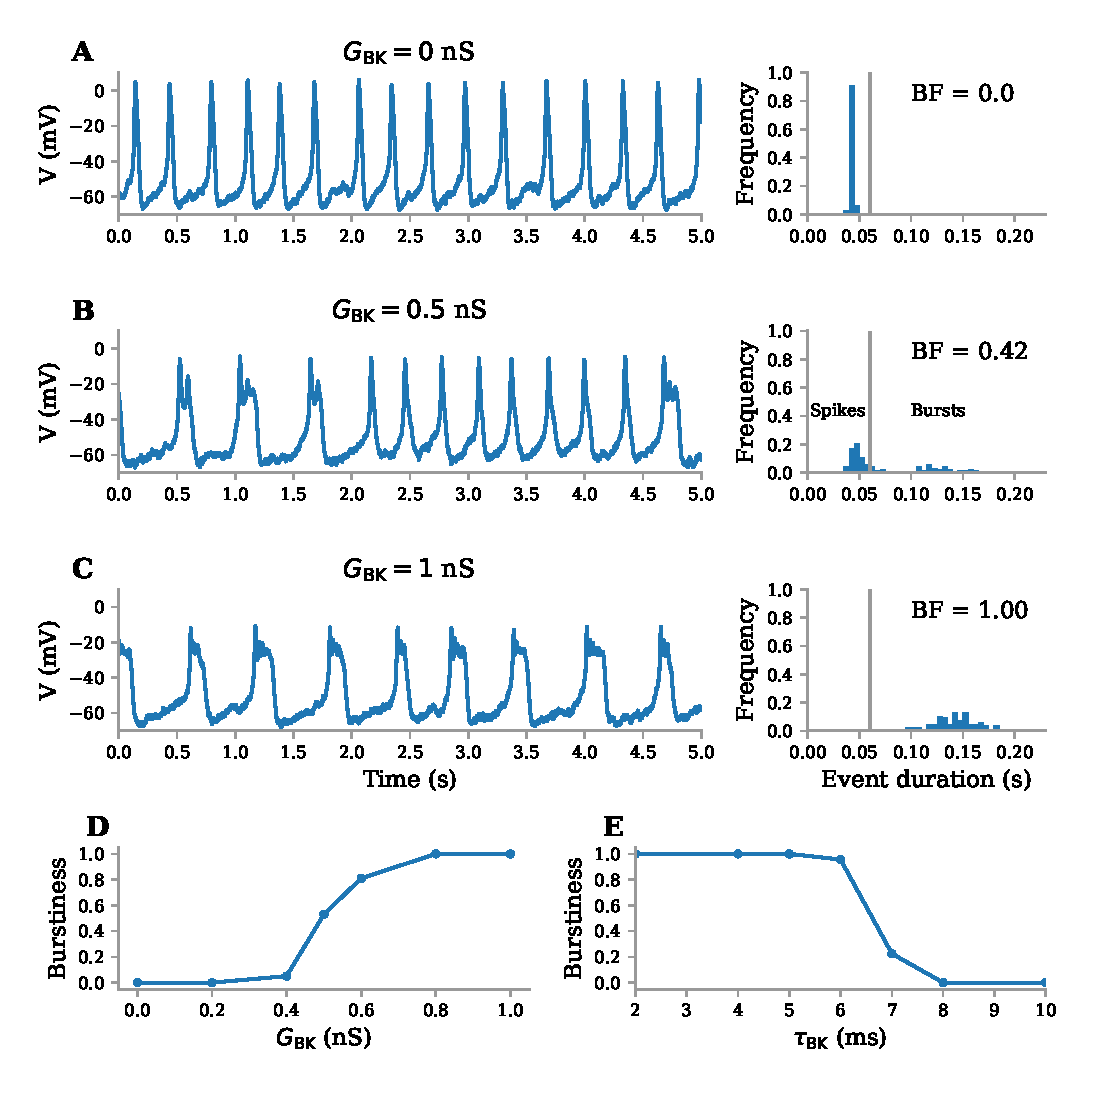
\includegraphics{figures/figure_1.eps}
\caption{Model predictions for the effect of various \(G_\mathrm{BK}\)
conductances on burstiness. \textbf{A}-\textbf{C} Left, membrane
potential of the model. Right, distribution of event durations in the
time interval from 1 to 5 s (of the 50 s simulated). The grey line
indicates the threshold for what is considered a spike and what is
considered a burst, and BF denotes the burstiness factor. \textbf{D} The
burstiness factor increased with \(G_\mathrm{BK}\). \textbf{E} The
burstiness factor decreased with
\(\tau_\mathrm{BK}\).}\label{fig:figure1}
\end{figure}

The results shown in Figure ~\ref{fig:figure2} correspond well to those
in Figure 2 of the original publication. In this figure,
\(G_\mathrm{BK}\) was fixed at a given value, while the remaining model
parameters were sampled randomly (see Methods). When \(G_\mathrm{BK}\)
was set to zero (Figure ~\ref{fig:figure2}\textbf{A}), most model
parameterizations had a low burstiness factor (between 0 and 0.1).
Oppositely, when \(G_\mathrm{BK}\) was fixed at the maximum value
(Figure ~\ref{fig:figure2}\textbf{C}), most model parameterizations had
a high burstiness factor (between 0.9 and 1). For any value of
\(G_\mathrm{BK}\), the model evaluations tended to be either
predominantly bursting (i.e.~most events were bursts) or predominantly
spiking (few events were bursts), so that the number of model
evaluations with an intermediate burstiness factor between 0.1 and 0.9
(events changed between being bursts or not) was always low (less than
20 evaluations).

Albeit qualitatively similar, the presented results were not strictly
identical to those in the original publication. As random noise was
added to the simulations, exact replications were unattainable, and some
discrepancies between the current and the original study were expected.
The largest deviations between the current analysis and the original
work were seen in Figure ~\ref{fig:figure1}\textbf{B} (right panel),
where the original work found a burstiness factor of 0.34, while our
analysis found a burstiness factor of 0.42, and in Figure
~\ref{fig:figure2}\textbf{C}, where the number of model evaluations with
a low burstiness factor was much higher (approximately 75) in the
original work compared to what we found in the current analysis (16).
Below, we analyze whether the observed discrepancies can be ascribed to
noise, or if they may reveal other differences in implementation
details. We limit the analysis to only consider the above mentioned two
cases.

\begin{figure}
\centering
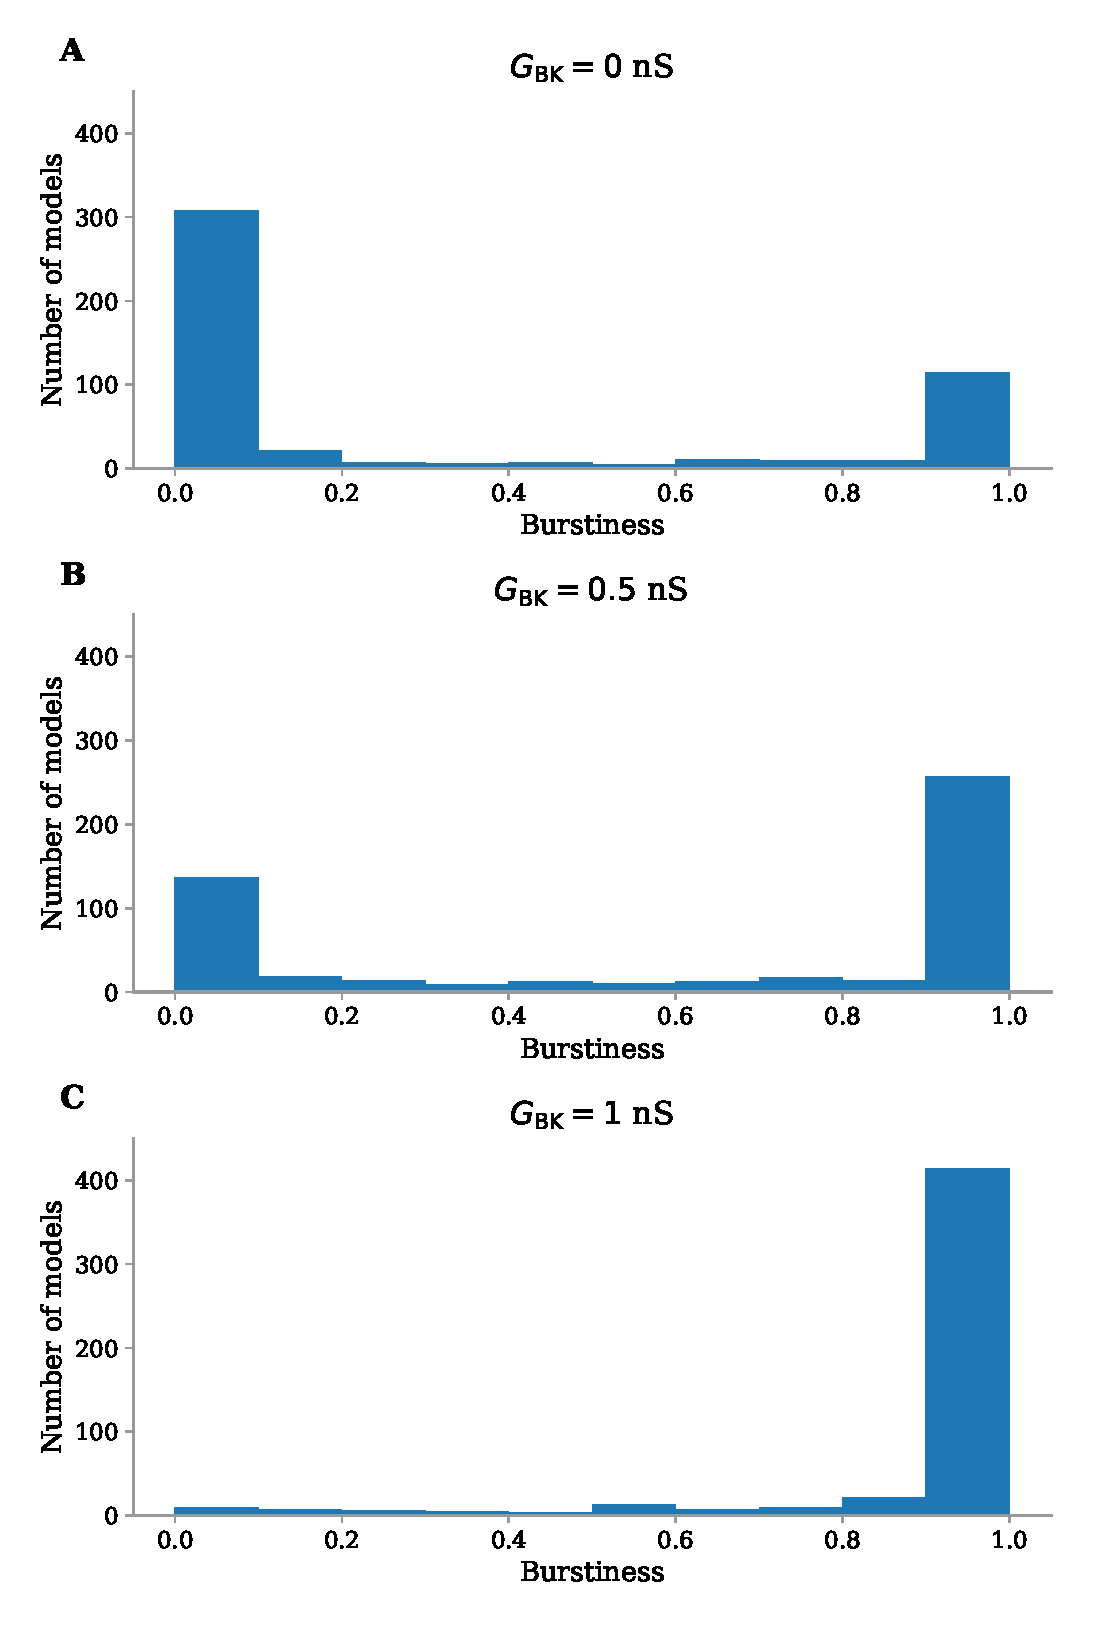
\includegraphics{figures/figure_2.eps}
\caption{Robustness of the burstiness of the model for three values of
\(G_{\mathrm{BK}}\) when changing \(G_{\mathrm{Ca}}\),
\(G_{\mathrm{K}}\), \(G_{\mathrm{SK}}\), and \(G_{\mathrm{l}}\)
uniformly within \(\pm 50\%\) of their original values. \textbf{A} For
\(G_{\mathrm{BK}} \rightarrow 0\) nS, \(67.5\%\) of the active models
were spikers (burstiness factor \(< 0.3\)). \textbf{B} For
\(G_{\mathrm{BK}} \rightarrow 0.5\) nS, \(33.8\%\) were spikers.
\textbf{C} For \(G_{\mathrm{BK}} \rightarrow 1\) nS, only \(4.4\%\) were
spikers.}\label{fig:figure2}
\end{figure}

\subsection{Examining the discrepancies between the replicated and
original
simulations}\label{examining-the-discrepancies-between-the-replicated-and-original-simulations}

Below, we examine whether the discrepancies between the current and
original work, as reflected in Figure ~\ref{fig:figure1}\textbf{B} and
Figure ~\ref{fig:figure2}\textbf{C}, can be explained by (i) the random
noise added in the simulations, (ii) differences in integration methods,
as reflected by the simulation time step dt, (iii) numerical floating
point errors introduced when converting from total conductances to
conductance per-unit-area by choosing a membrane area A, or if (iv) the
discrepancies may reflect unintended differences in the algorithms for
the model analysis.

We start by exploring the burstiness factor (BF) in Figure
~\ref{fig:figure1}\textbf{B}, which reflects the fraction of events that
were bursts in a single simulation. As the burstiness factor varies from
simulation to simulation (due to noise), we calculated it for 100 reruns
of the model, which allowed us to calculate its mean and standard
deviation (Figure ~\ref{fig:burstinessfactor}). We calculated the mean
and standard deviations for three different values of the area
(\(A = \pi\cdot 10^{-9}; \pi \cdot 10^{-6}; \pi \cdot 10^{-3}\)) , and
three values of the timestep (\(\mathrm{dt} = 0.05; 0.005; 0.001\)), and
the obtained statistics did not vary much with these model choices. In
all cases, the burstiness factor had a mean of about 0.4 and a standard
deviation of about 0.04. The burstiness factor of 0.34 found in the
original work was thus roughly a standard deviation lower than the mean
found here, and it is thus not too unlikely that the observed
discrepancies could be due to random noise (i).

\begin{figure}
\centering
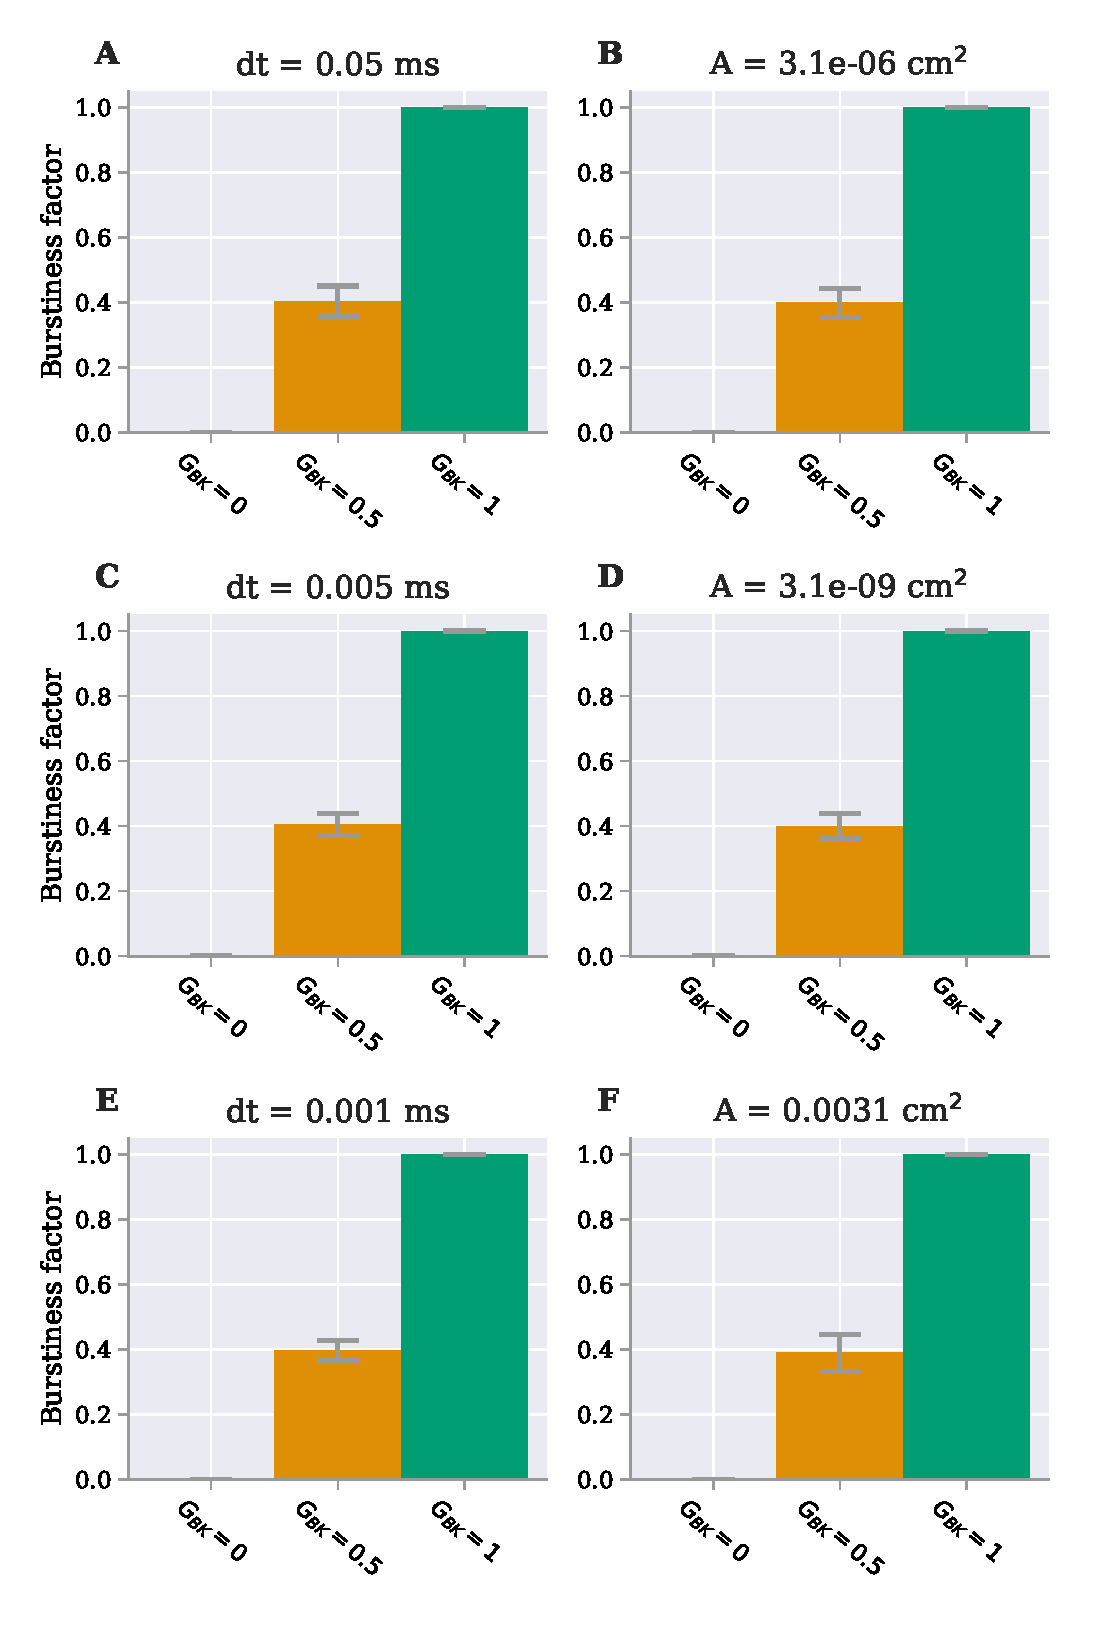
\includegraphics{figures/burstiness_factor.eps}
\caption{Mean and standard deviation of the burstiness factor of 100
reruns of the model for three values of the area (A), three values of
the timestep ((\(\mathrm{dt}\)), and three values of
\(G_{\mathrm{BK}}\). Panel \textbf{B} shows the results for model using
the original parameters.}\label{fig:burstinessfactor}
\end{figure}

Next, we explored how the results presented in Figure
~\ref{fig:figure2}\textbf{C} depended on the choice of membrane area and
simulation time step. Figure ~\ref{fig:dtarea} shows the burstiness of
the model for three values of the area
(\(A = \pi\cdot 10^{-9}, \pi \cdot 10^{-3}, 1\)) and three values of the
timestep (\(\mathrm{dt} = 0.05, 0.005, 0.001\)), changing one of them at
the time. When comparing Figure ~\ref{fig:dtarea} to Figure
~\ref{fig:figure2}\textbf{C} we see that changes in either the timestep
or the area causes very little changes in the overall results. The small
variations between the different panels in Figure ~\ref{fig:dtarea} are
thus most likely due to the random noise. In this case, neither noise
(i), integration method differences (ii), or floating point errors (iii)
seem like a likely explanation of the discrepancies between the original
simulation and the current results.

\begin{figure}
\centering
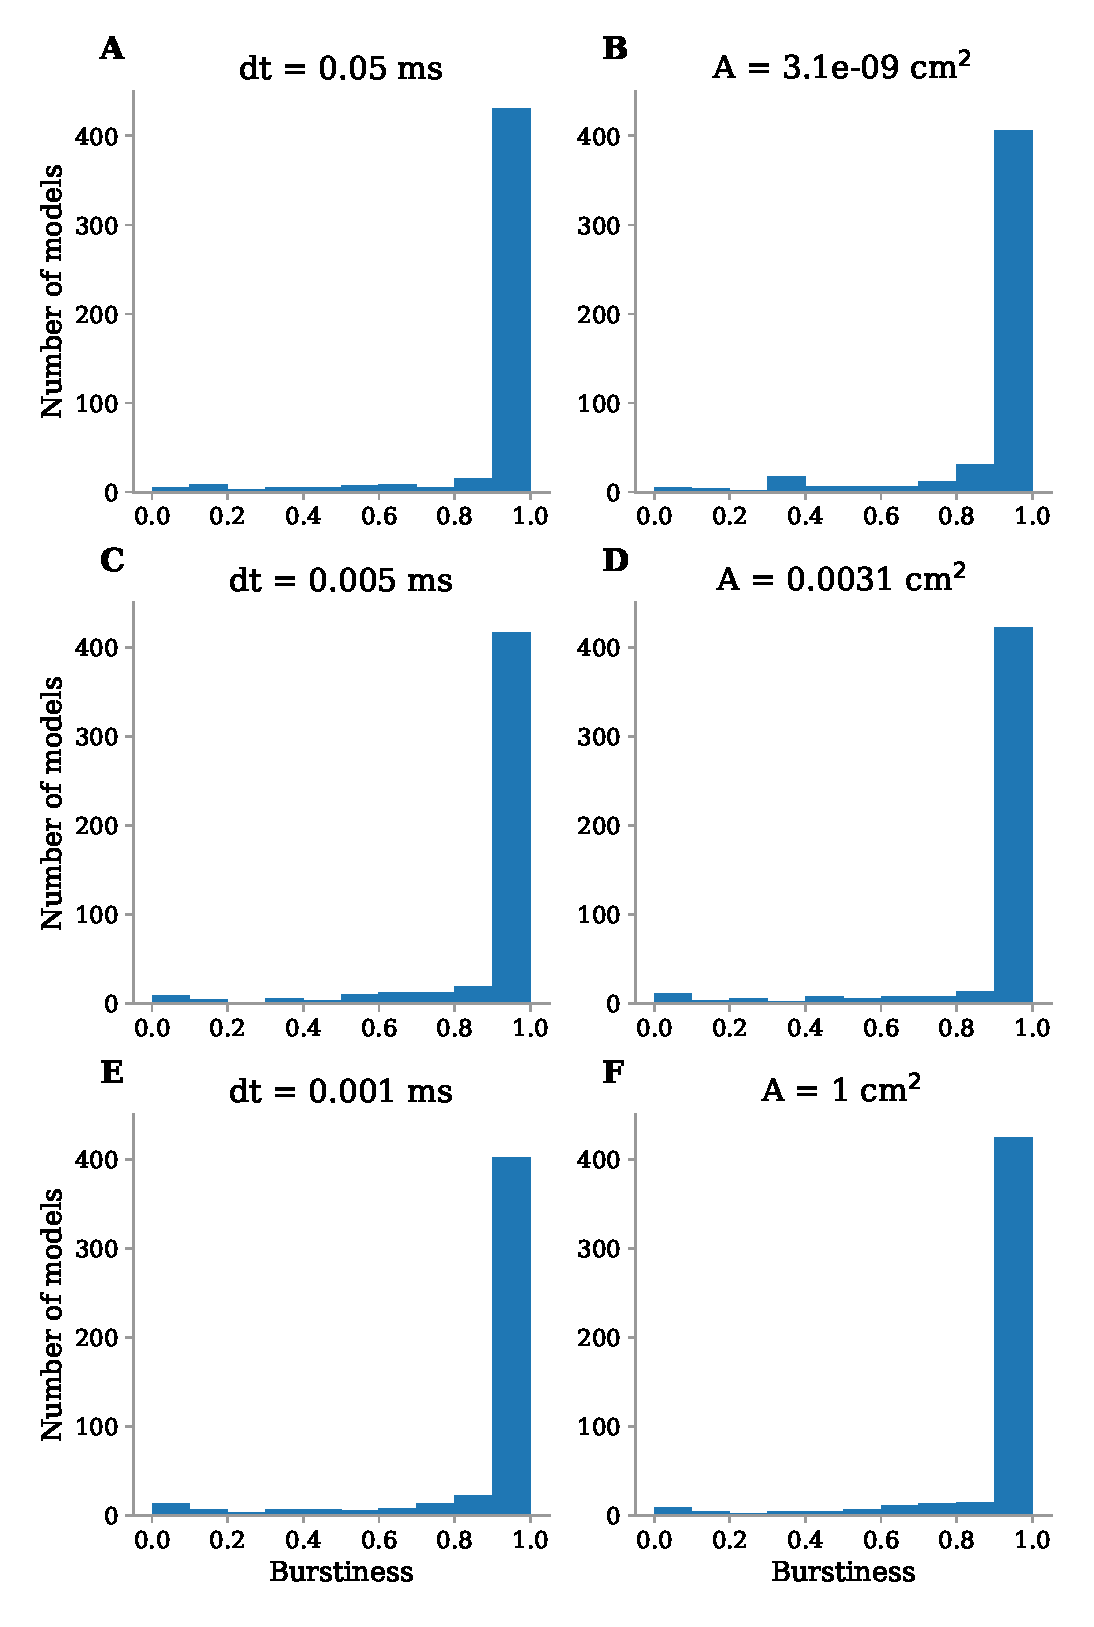
\includegraphics{figures/dt_area.eps}
\caption{Burstiness of the model for three values of the area and three
values of the timestep when changing \(G_{\mathrm{Ca}}\),
\(G_{\mathrm{K}}\), \(G_{\mathrm{SK}}\), and \(G_{\mathrm{l}}\)
uniformly within \(\pm 50\%\) of their original values. When changing
the area the timestep was kept unchanged at \(\mathrm{dt} = 0.01\) and
when changing the timestep the area was kept unchanged at
\(\pi \cdot 10^{-6}\). \(G_{\mathrm{BK}} = 1\) as that is where we
observed the difference.}\label{fig:dtarea}
\end{figure}

The above indicates that there might be some small differences between
the current and original implementation that are not due to noise or
numerical issues (iv). We were not able to detect the precise cause of
the observed difference. We believe that the model itself is identical
in the two cases (we have compared our code with the XPP code from the
original work \autocite{tabak2011}) and that the differences are more
likely to reflect differences in the choices made in the analysis part.
These could be choices regarding event detection (such as the definition
of onset and termination thresholds and burst definition), or criteria
for which simulations that were included in and discarded from the
analyses. These choices were imprecisely described in the original work,
and it is possible that we have made some minor misinterpretations, and
that our criteria deviate slightly from the original ones. In the
original work, the robustness results (Figure 2) in the original
publication were calculated using custom developed software that used
CUDA to run on GPUs, and the code for performing this analysis was not
available.

\subsection{Uncertainty quantification and sensitivity
analysis}\label{uncertainty-quantification-and-sensitivity-analysis-1}

The uncertainty quantification and sensitivity analysis of the model is
shown in Figure ~\ref{fig:sensitivity}. The sensitivity was given as the
total-order Sobol indices, which quantify how much of the variance of
the model each parameter (accounting for all of its interactions with
other parameters) is responsible for \autocite{homma1996}.

\begin{figure}
\centering
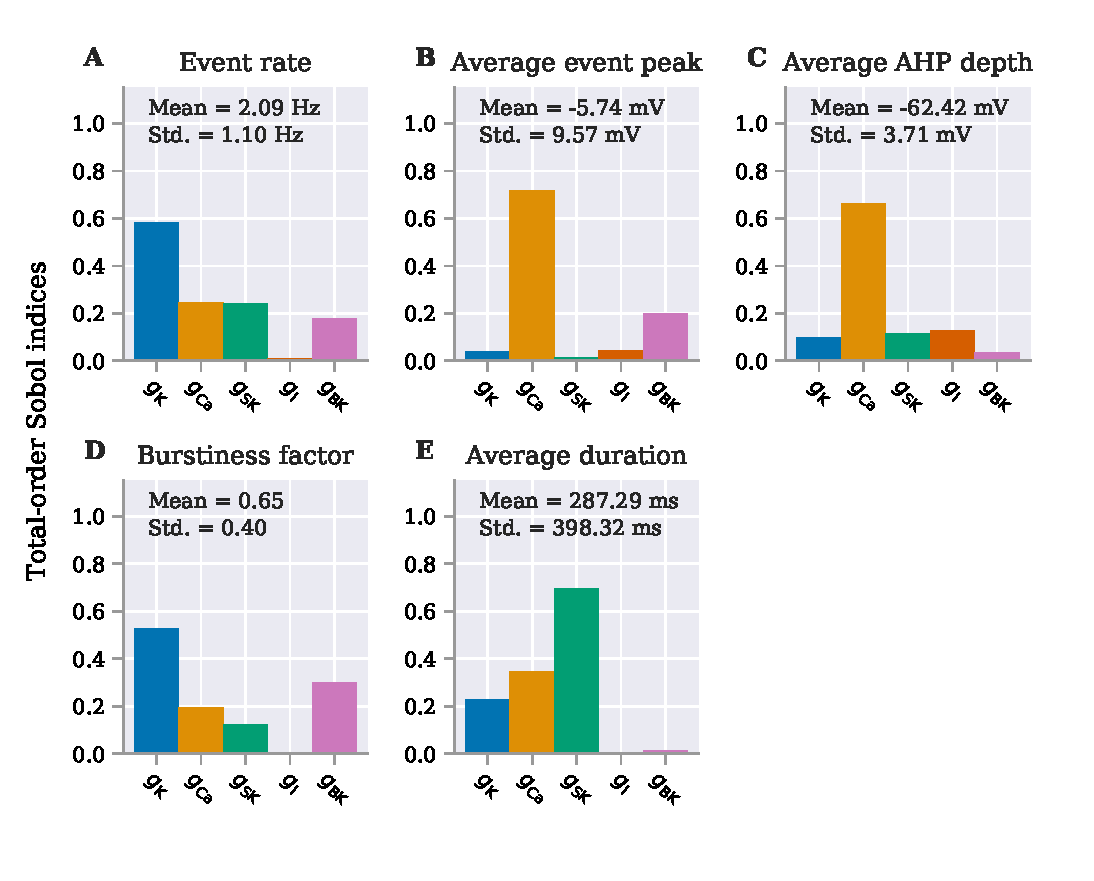
\includegraphics{figures/sensitivity.eps}
\caption{Uncertainty quantification and sensitivity analysis of a
selected set of response features of the model. \textbf{A} Event rate
denotes the event firing rate. \textbf{B} Average event peak denotes is
the average event peak voltage. \textbf{C} Average AHP
(afterhyperpolarization) depth denotes the average minimum voltage
between two consecutive events. \textbf{D} Burstiness factor denotes the
fraction of events with duration longer than 60 ms. \textbf{E} Average
duration denotes the average duration of the
events.}\label{fig:sensitivity}
\end{figure}

The sensitivity analysis showed that the spike rate was sensitive to
almost all ion channel conductances, but most so to \(G_{\mathrm{K}}\)
(Figure ~\ref{fig:sensitivity}\textbf{A}). Such a role of the delayed
rectifying K\textsuperscript{+} channel in controlling the firing rate
has been seen in other studies \autocite{guan2013}.

The event amplitude was mainly sensitive to \(G_{\mathrm{Ca}}\) (Figure
~\ref{fig:sensitivity}\textbf{B}), which is not surprising given that
the events are generated by \(I_{\mathrm{Ca}}\). However, it also had a
relatively high sensitivity to \(G_{\mathrm{BK}}\), in line with what
was found in the previous study \autocite{tabak2011}.

The average afterhyperpolarization depth was in turn most sensitive to
\(G_{\mathrm{Ca}}\) (Figure ~\ref{fig:sensitivity}\textbf{C}). This may
seem counterintuitive, as \(I_{\mathrm{Ca}}\) is not a hyperpolarizing
current. However, \(I_{\mathrm{Ca}}\) is responsible for triggering all
the three hyperpolarizing currents (\(I_\mathrm{K}\), \(I_\mathrm{BK}\)
and \(I_\mathrm{SK}\)) that generate the afterhyperpolarization depth.
\(I_\mathrm{K}\) and \(I_\mathrm{BK}\) are activated by the voltage
deflection caused by \(I_{\mathrm{Ca}}\), while \(I_\mathrm{SK}\) is
activated by the Ca\textsuperscript{2+} entering through
\(I_{\mathrm{Ca}}\).

The burstiness factor of the model was mainly sensitive to
\(G_{\mathrm{K}}\) and \(G_{\mathrm{BK}}\) (Figure
~\ref{fig:sensitivity}\textbf{D}). The sensitivity to
\(G_{\mathrm{BK}}\) confirms the findings in the original publication,
i.e.~that BK channels promote bursting. However, the large sensitivity
to \(G_{\mathrm{K}}\) is a novel insight for the current study and
indicates that also \(G_{\mathrm{K}}\) was important for determining if
the model produced bursts or spikes. This observation is tightly related
to the explanation for how BK can act as a burst promoter in the first
place, which is contrary to what one would expect from a hyperpolarizing
current. The explanation, proposed by both Tabak et al.
\autocite{tabak2011} and the experimental studies they were inspired by
\autocite{vangoor2001}, was that \(G_{\mathrm{BK}}\) promoted bursting
by reducing the peak amplitude of events (as reflected in Figure
~\ref{fig:sensitivity}\textbf{B}), thereby preventing full activation of
the otherwise more strongly hyperpolarizing delayed rectifier current
(\(I_{\mathrm{K}}\)). In this context, the sensitivity analysis simply
shows that the indirect effect on \(I_{\mathrm{K}}\) obtained by varying
\(G_{\mathrm{BK}}\) was smaller than the direct effect on
\(I_{\mathrm{K}}\) obtained by varying \(G_{\mathrm{K}}\) (Figure
~\ref{fig:sensitivity}\textbf{D}).

Surprisingly, the average event duration had a very low sensitivity to
\(G_{\mathrm{BK}}\) (Figure ~\ref{fig:sensitivity}\textbf{E}), and was
instead most sensitive to \(G_{\mathrm{SK}}\). This was unexpected since
the burstiness was highly sensitive to \(G_{\mathrm{BK}}\), and a burst
was defined as an event exceeding a certain duration. An exploration of
the counterintuitive relationship between Figure
~\ref{fig:sensitivity}\textbf{D} and \textbf{E} is presented below.

\subsection{Parameter exploration}\label{parameter-exploration}

To explore the relationship between the results in Figure
~\ref{fig:sensitivity}\textbf{D} and \textbf{E}, we examined the effects
of varying \(G_\mathrm{BK}\), \(G_{\mathrm{K}}\), and
\(G_{\mathrm{SK}}\) on the burstiness and the average duration of events
(Figure ~\ref{fig:durations}). It should be noted that this figure only
shows how the model responds when changing two parameters at the time,
so the higher-order interactions included in the total-order Sobol
sensitivity indices are absent.

\begin{figure}
\centering
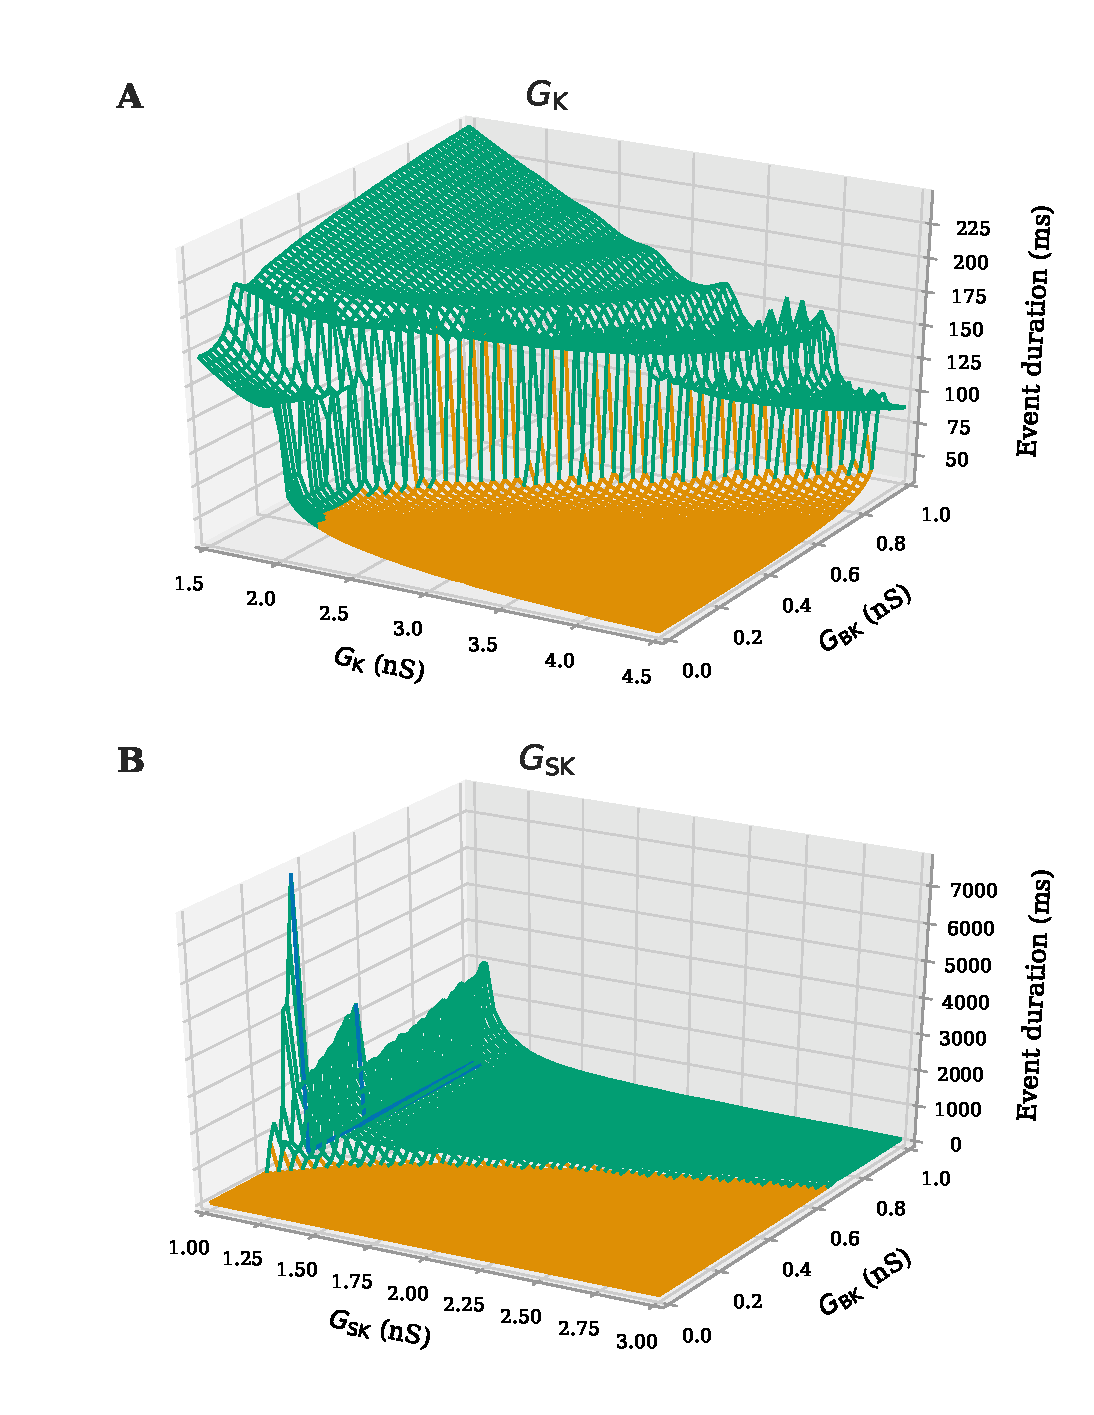
\includegraphics{figures/durations.eps}
\caption{The average duration of events while varying \(G_\mathrm{BK}\)
and either \textbf{A} \(G_{\mathrm{K}}\) or \textbf{B}
\(G_{\mathrm{SK}}\). The areas in parameter space where the average
duration of the events is longer than the burstiness factor threshold
are in green, while the areas where the average duration is below this
threshold are in yellow. Areas in blue produce no events and the average
duration is then set to -1 for visualization
purposes.}\label{fig:durations}
\end{figure}

Figure ~\ref{fig:durations}\textbf{A} shows the regions in the
\(G_{\mathrm{BK}}\)/\(G_{\mathrm{K}}\) parameter plane where the model
produced regular spikes (yellow) and bursts (green). For low (\(<\) 2
nS) values of \(G_{\mathrm{K}}\), the cell was bursting regardless of
the value of \(G_{\mathrm{BK}}\). Hence, for low values of
\(G_{\mathrm{K}}\), the burstiness of the cell was insensitive to
\(G_{\mathrm{BK}}\). In comparison, a sufficiently large change in
\(G_{\mathrm{K}}\) could switch the cell between a regular and bursty
state for any (fixed) value of \(G_{\mathrm{BK}}\). These results thus
fit well with the sensitivity analysis in Figure
~\ref{fig:sensitivity}\textbf{D}, which showed that the burstiness was
more sensitive to \(G_{\mathrm{K}}\) than to \(G_{\mathrm{BK}}\).

We next fixed \(G_{\mathrm{K}}\) at the default value 3 nS, and explored
how it could be the case that burstiness was sensitive to
\(G_{\mathrm{BK}}\) but not so much to \(G_{\mathrm{SK}}\), while event
duration was sensitive to \(G_{\mathrm{SK}}\) but not so much to
\(G_{\mathrm{BK}}\) (Figure ~\ref{fig:durations}\textbf{B}). As the
figure shows, for \(G_{\mathrm{BK}}<\) 0.2 nS the cell was always
regularly spiking, while for \(G_{\mathrm{BK}}>\) 0.8 nS, the cell was
always bursting, irregardless of the values of \(G_{\mathrm{SK}}\). In
comparison, changing \(G_\mathrm{BK}\) (keeping \(G_{\mathrm{SK}}\)
fixed) could always switch the cell between a regular and bursty state.
In equivalence with the analysis of Figure
~\ref{fig:durations}\textbf{A}, this explains why the burstiness was
less sensitive to \(G_{\mathrm{SK}}\) than \(G_{\mathrm{BK}}\). However,
although changes in \(G_{\mathrm{BK}}\) more often led to changes in
burstiness, the effects on the event duration was modest. That is, for
most (fixed) values of \(G_{\mathrm{SK}}>\), a change in
\(G_{\mathrm{BK}}\) could push the event duration from slightly below to
slightly above the burst-duration threshold, but did not lead to larger
changes in burstiness. Oppositely, reducing \(G_\mathrm{SK}\) to the
lower values in the explored range resulted in burst durations of
several thousands of milliseconds (as long as \(G_{\mathrm{BK}}>\) 0.2
nS). Hence, while \(G_{\mathrm{BK}}\) was important for achieving a
burst in the first place, \(G_{\mathrm{SK}}\) had a much larger impact
on the duration of the burst. This explains the difference in
sensitivity between the average duration and burstiness factor observed
in Figure ~\ref{fig:sensitivity}\textbf{D} and \textbf{E}.

\section{Conclusion}\label{conclusion}

We were able to qualitatively reproduce all the computational results in
Tabak et al. \autocite{tabak2011}. By performing an uncertainty
quantification and sensitivity analysis we confirmed the key conclusions
in the original publication using a different simulator and different
analysis methods, which provided additional insight into how different
membrane mechanisms interact to produce the characteristic response
features of the model. Overall, the reproduction effort went smoothly,
with a little help from the original authors in describing the
threshold-detection algorithm used in the analysis of the model. The
original model now exists as a model using the Python interface for
NEURON, which hopefully makes it accessible to a wider audience. Our
personal motivation for reproducing the model by Tabak et al. was that
we needed it in a computational study where we compared the dynamical
properties of pituitary cells in rats versus fish \autocite{halnes2018}.

{\sffamily \small
  \printbibliography[title=References]
}
\end{document}
